\section{Proposed Design}
\label{section:propeseddesign}

Before doing any implementation, we conducted some investigation into how Hadoop works, 
specifically how it assigns tasks initially and how they are reassigned during runtime.
These are important attributes to understand, because they contribute to uneven effective
workloads in a heterogeneous environment; that is, if two machines are assigned equal-sized
tasks, but one machine is twice as powerful as the other, it was effectively given half as
much work since it will complete it twice as fast as the other machine.

\subsection{Hadoop MapReduce Task Assignment}

We show the steps Hadoop MapReduce takes to carry out a job in \ref{fig:flow}. There are
three primary pieces to a MapReduce application: the user application defining the kind of job
to be executed, the Distributed File System (DFS), and the hadoop core framework that executes
the Map and Reduce Tasks on the input data. MapReduce 
works by first allowing the user application (such as Wordcount) to define map and reduce functions
from the application.
Next the user application configures a \texttt{Job} object representing that application and its configuration.
Input data for the job is loaded into the Hadoop Distributed File System by the user. 
The job is then submitted to the \texttt{JobClient}, which acts as the interface between the user
application and the Hadoop framework. Subsequently, the JobClient calls the 
\texttt{getSplits} method to divide the input data to appropriate sizes to be executed on MapTasks. The job and
input splits are submitted to the \texttt{JobTracker}, which is responsible for managing the \texttt{TaskTrackers} and assigning them
tasks. The \texttt{TaskTracker} on each slave node communicates with
the \texttt{JobTracker} on the master node by sending it a "Heartbeat" which indicates it's status. If the \texttt{TaskTracker}
has open slots, the \texttt{JobTracker} will assign it tasks and FileInput splits. The jobqueue is maintained by the
\texttt{TaskScheduler} which is responsible for this assignment. Finally, once the \texttt{TaskTracker} is finished
with a task, its output is written back to the DFS.

\begin{figure}[ht!]
\centering
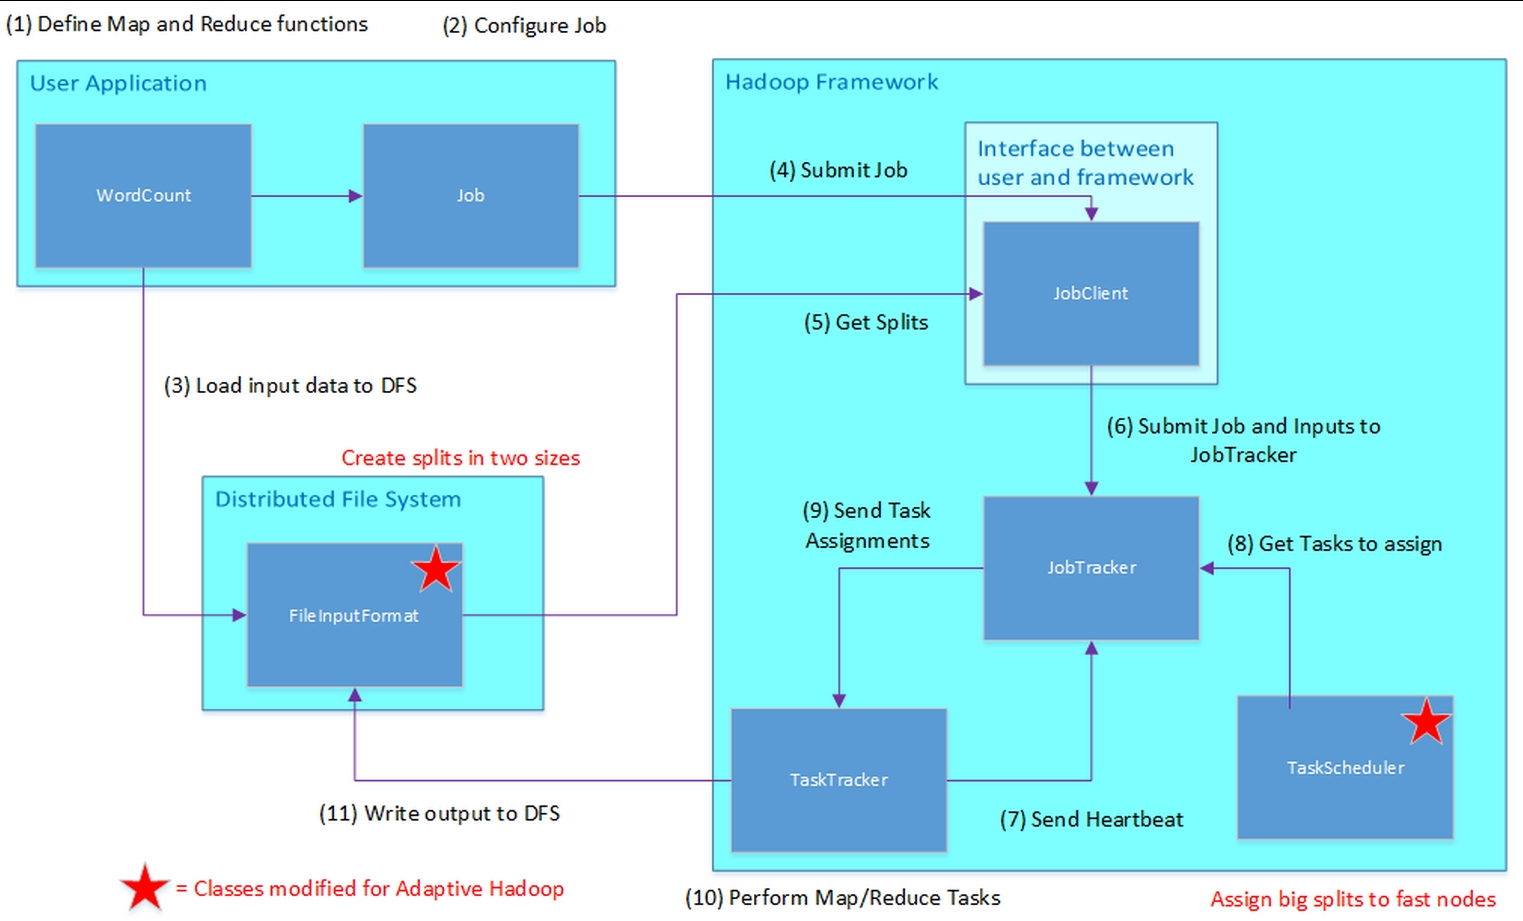
\includegraphics[width=90mm]{flow.jpg}
\caption{Workflow of a Hadoop MapReduce job}
\label{fig:flow}
\end{figure}

\begin{figure}[ht!]
\centering
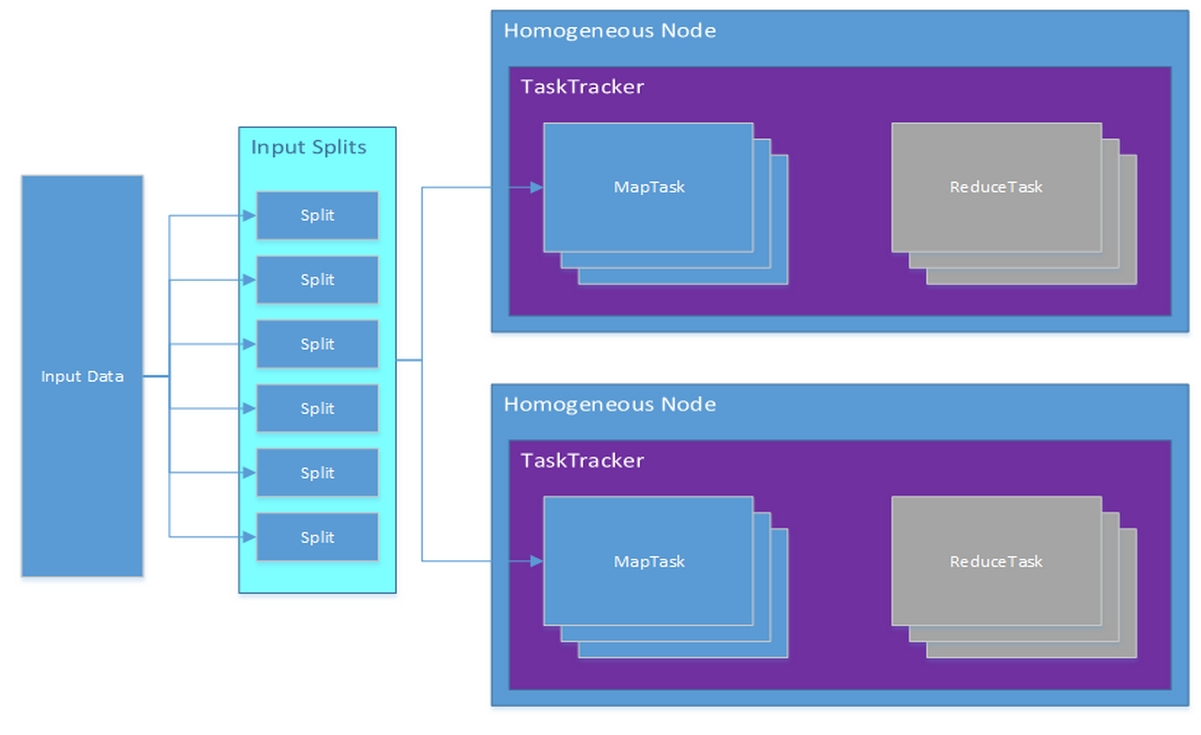
\includegraphics[width=90mm]{homogeneous_mr.jpg}
\caption{MapReduce task assignment in Homogeneous Environment}
\label{fig:homogeneoues_mr}
\end{figure}

\begin{figure}[ht!]
\centering
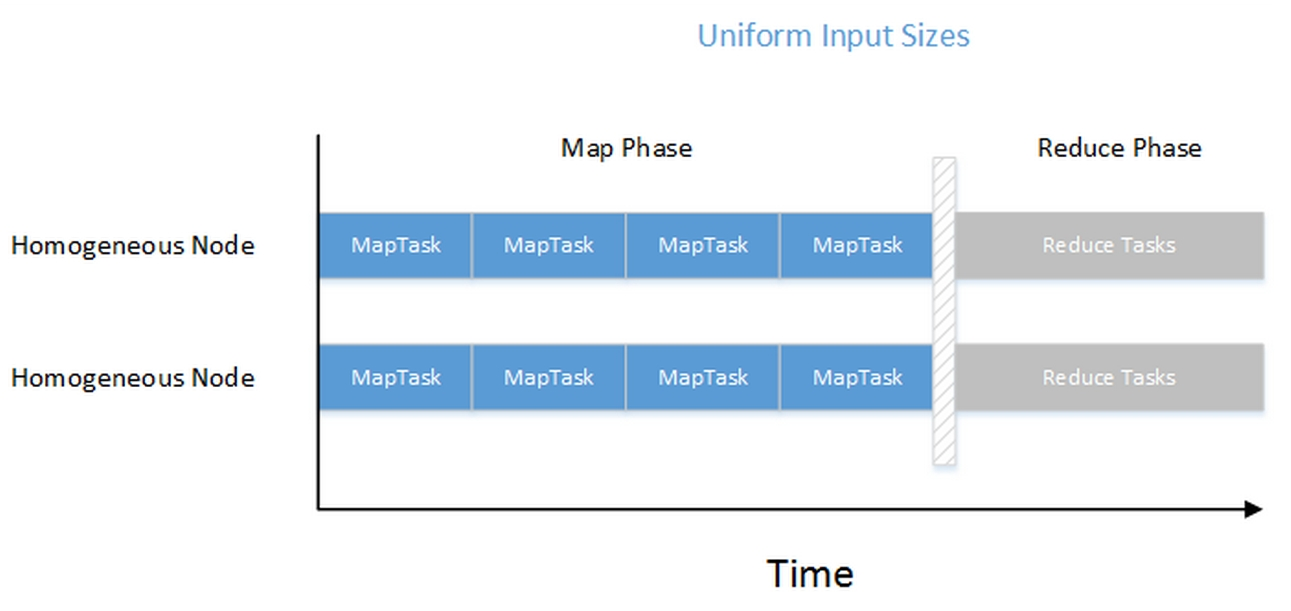
\includegraphics[width=90mm]{homogeneous_time.jpg}
\caption{MapReduce task completion in Homogeneous Environment}
\label{fig:homogeneoues_time}
\end{figure}

Hadoop MapReduce is designed for homogeneous environments. Without modifications, when Hadoop receives a job,
it first takes the input files and divides them into evenly-size splits that
get written back to the DFS (Distributed File System). In a homogeneous configuration, the Hadoop cluster
will have multiple nodes with similar hardware capabilities. Each of these slave nodes will have a
TaskTracker that is responsible for running and monitoring the MapTasks and ReduceTasks. During the MapPhase,
when the TaskTracker has open map slots available, it will execute MapTasks with the input splits that were
created before. This structure is depicted in \ref{fig:homogeneous_mr}.


\ref{fig:homogeneous_time} illustrates how these MapTasks execute in a homogeneous environment. Since the homogeneous nodes have
similar hardware and processing capabilities, they should execute their tasks in relatively the same amount of
time given the same number of MapTasks with the same input sizes. This is the ideal case and the most efficient use of cluster hardware.
. 


Modern datacenters, as we discussed in \ref{motivation}, are usually heterogeneous. That means,
when given the same amount of uniformly-sized tasks, different nodes will complete their tasks 
at different times. Since the nodes
have different processing capabilities, some of the nodes will finish their MapTasks faster than others
resulting in uneven overall execution time. Since the Reduce phase and tasks cannot begin until all of
the MapTasks are completed, this leaves some idle time for the nodes that have completed their tasks and
are waiting for the slower nodes to catch up. We show an example of this in \ref{fig:heterogeneous_time}.
If the task completion
is skewed enough, the fastest nodes will actually steal tasks from the slower nodes; however,
this would introduce other performance issues from the overhead of the task stealing, and
sub-optimal performance from potential data locality issues. We believe a better solution is to
adjust the FileInput split sizes in proportion to the nodes' performance capabilities, such that
the total task completion time for each node is the more balanced (\ref{adaptive_mr}). We could do this by making some larger
splits which would be assigned to the more powerful nodes. \ref{adaptive_time} shows the execution of this optimal adaptation. Even though the nodes have different processing
capabilities, if they also have proportionately different input sizes then their overall execution should balance out.

\begin{figure}[ht!]
\centering
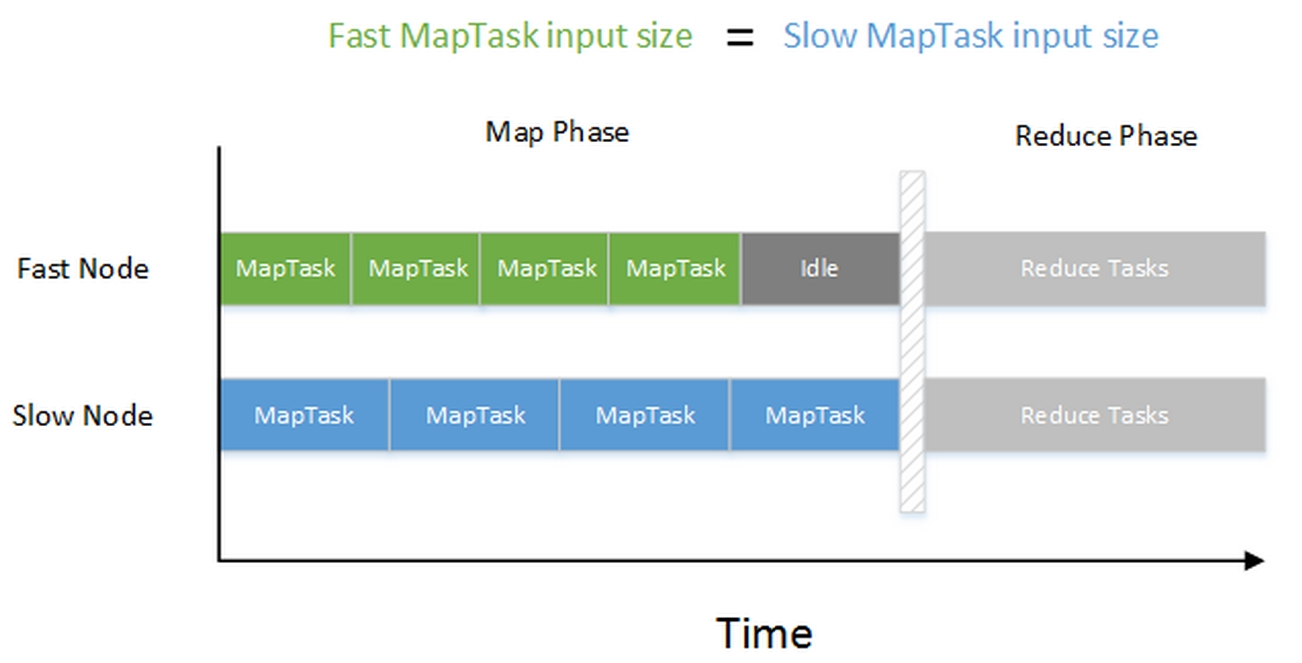
\includegraphics[width=90mm]{heterogeneous_time.jpg}
\caption{MapReduce task completion in Heterogeneous Environment}
\label{fig:heterogeneous_time}
\end{figure}

\begin{figure}[ht!]
\centering
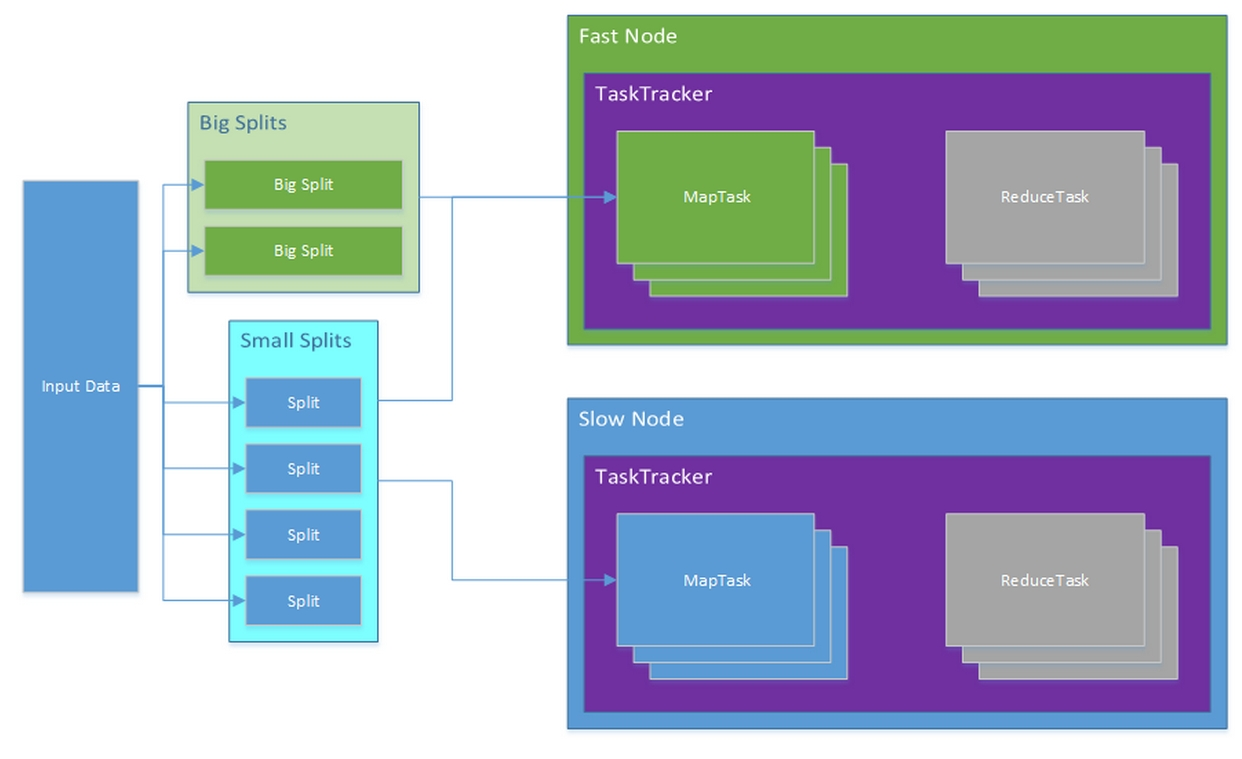
\includegraphics[width=90mm]{adaptive_mr.jpg}
\caption{MapReduce adapted flow for Heterogeneous Environment}
\label{fig:adaptive_mr}
\end{figure}

\begin{figure}[ht!]
\centering
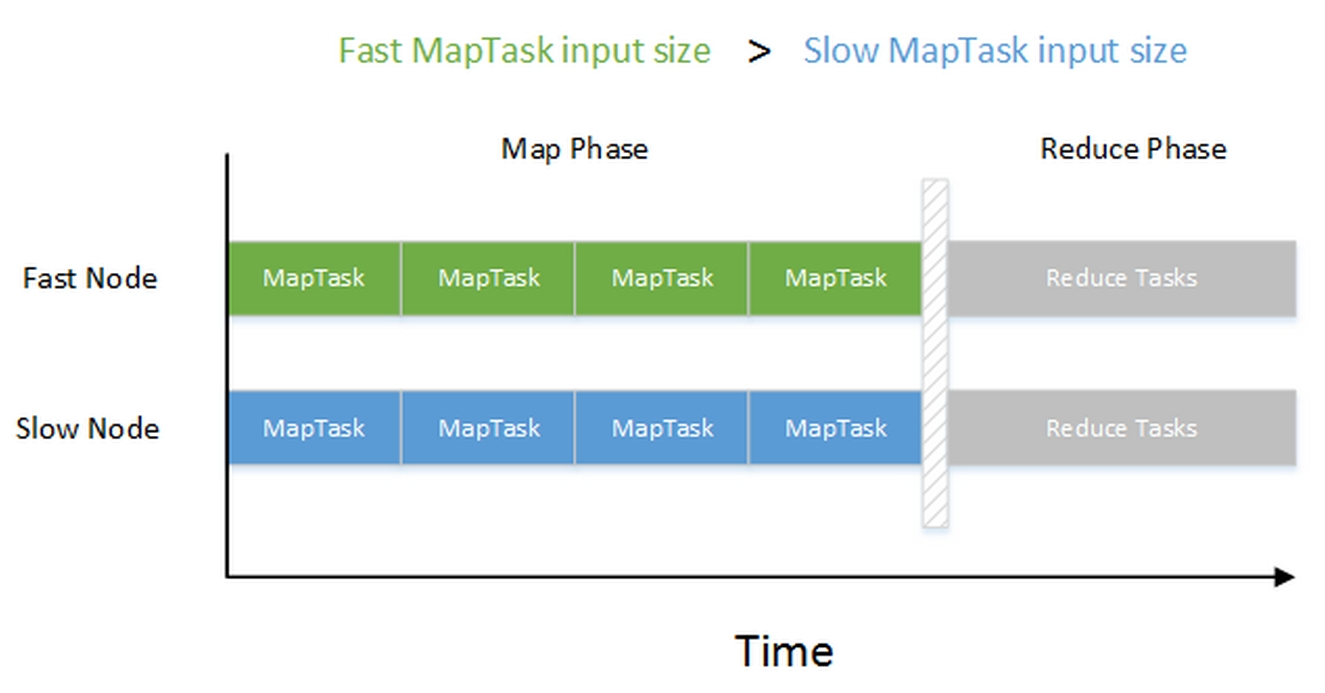
\includegraphics[width=90mm]{adaptive_time.jpg}
\caption{MapReduce task completion in Heterogeneous Environment with adaptive split sizes}
\label{fig:adaptive_time}
\end{figure}

\subsection{Datacenter VM Interference}
\label{sec:interference}
In addition to hetergeneous machines, datacenters can also exhibit temporal heterogeneity.
VM performance depends on the behavior of other VMs on the same machine at any given time.
This means a VM on a machine with other, inactive VMs will initially be very performant;
but once the other VMs begin doing work the VM will experience performance degradation.
The variability of a VM's performance also depends on the abstraction layer between the VMs
and the physical hardware.

\subsection{Hadoop MapReduce Task Stealing}
The hardware interefence described in \ref{sec:interference} must be addressed dynamically
during runtime. An intuitive place to insert extra logic addressing this is during task
stealing.

In MapReduce jobs, each node is typically assigned a number of tasks. As some nodes 
complete their work ahead of schedule, they will steal tasks from other, backed-up,
nodes. If we modified the logic around which nodes to steal from, and how much work
to steal, we could help ensure all the tasks are finished closer to the same time.

